\chapter{Evaluation}
\thispagestyle{plain}

\label{Evaluation}

To evaluate the approaches developed, we processed web pages using Kuhn's tool, SPRWeb and our tool and then compared the web pages on factors such as naturalness, differentiability, subjective naturalness and subjective differentiability.

\section{Improvements in SPRWeb}
\label{Improvements in SPRWeb}
We compared our tool with Kuhn’s[8] re-coloring tool.  Metrics of comparison were perceptual naturalness, perceptual differentiability, subjective naturalness and subjective differentiability as defined in definitions section in Chapter 2. 

\begin{table}[!htb]
\caption{Evaluation: Improvements in SPRWeb (numbers in scaled CIELAB euclidean distance)}
% title of Table
\centering
% used for centering table
\begin{tabular}{c c c c c c c c c}
% centered columns (4 columns)
\hline\hline
%inserts double horizontal lines
Web Page & N-k & N-t & D-k & D-t & SN-k & SN-t & SD-k & SD-t\\ [0.5ex]
% inserts table
%heading
\hline
% inserts single horizontal line
Complex 1 & 34 & 16 & 18 & 2.64 & 0.87 & 0.5 & 0.05 & 0.2 \\
% inserting body of the table
Complex 2 & 23 & 10 & 12 & 2.11 & 0.84 & 0.6 & 0.02 & 0.3\\
Complex 3 & 30 & 11 & 14 & 0.7 & 0.88 & 0.4 & 0.05 & 0.1\\
Complex 4 & 50 & 3 & 50 & 0.5 & 4 & 0.08 & 3.5 & 0.02\\
Complex 5 & 50 & 16 & 50 & 4.5 & 4 & 0.6 &1.3 & 0.2\\
Complex 6 & 33 & 8 & 20 & 0.3 & 1.23 & 1.04 & 0.14 & 0.3\\
Complex 7 & 47 & 16 & 17 & 2.15 & 0.87 & 1.01 & 0.018 & 0.4\\
Complex 8 & 50 & 27 & 20 & 4.25 & 1.73 & 1.5 & 1.37 & 0.4\\
Complex 9 & 40 & 21 & 23 & 4 & 0.99 & 1.1 & 0.1 & 0.5\\
Complex 10 & 50 & 21 & 50 & 2.6 & 3.07 & 1.1 & 4 & 0.3\\
Complex 11 & 18 & 6 & 15 & 1.6 & 0.78 & 0.4 & 0.05 & 0.2\\
Complex 12 & 44 & 17 & 17 & 3.8 & 1.29 & 0.6 & 0.02 & 0.2\\
Complex 13 & 27 & 12 & 23 & 1.7 & 0.8 & 0.7 & 0.15 & 0.3\\
Complex 14 & 14 & 4 & 10 & 0.5 & 0.3 & 0.1 & 0.104 & 0.1\\ [1ex]
% [1ex] adds vertical space
\hline
%inserts single line
\end{tabular}
\label{table:nonlin}
\begin{tabular}{@{}>{$}l<{$}l@{}}
    $k$ & Kuhn's Tool\\
    $t$ & Our tool developed by improvements in SPRWeb\\
    $N$ & Naturalness\\
    $D$ & Differentiability\\
    $SN$ & Subjective Naturalness\\
    $SD$ & Subjective Differentiability\\
  \end{tabular}
% is used to refer this table in the text
\end{table}

First we converted the output colors obtained from both kuhn's[8] and our tool to CIELAB notation. To assess naturalness-preservation, we compared the L*a*b* Euclidean distance between each original color and its respective Kuhn[8] and our replacement colors. Lower distances represent better naturalness-preservation, i.e., the replacement color is more perceptually-similar to the original color.To test perceptual differentiability, we calculated the Euclidean distance between each pair of colors in each original website and determined the absolute difference between this distance and the equivalent color pair in the Kuhn[8] and our versions. Lower values represent better differentiability restoration, i.e., the replacement colors are as differentiable (not more or less differentiable) as the original colors. Fig 4.1 gives a better view of comparison of the two tools in perceptual factors. 

\begin{figure}[!htb]
\centering
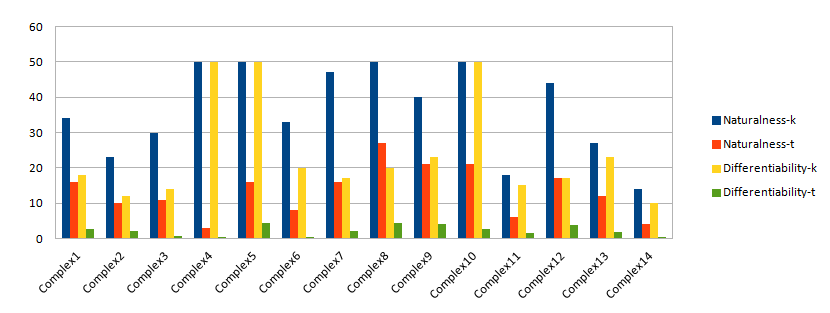
\includegraphics[width=\linewidth]{bar1.png}
\caption{Perceptual factors comparison}
\label{fig:sub2}
\end{figure}

For theoretical subjective response, we followed the same procedure as in the case of perceptual factors. The major difference being that instead of using $L^{*}$,$a^{*}$ and $b^{*}$ as three dimensions, we used temperature, activity and weight as three dimensions to represent colors (as defined in chapter 2). For each of the color in original CSS, kuhn's[8] solution and our solution, we calculated the temperature, activity and weight factors. Then these three values are taken as one coordinate and same process as followed in  perceptual factors was followed. Fig 4.2 compares kuhn's tool and our tool in subjectivity measures. 

\begin{figure}[!htb]
\centering
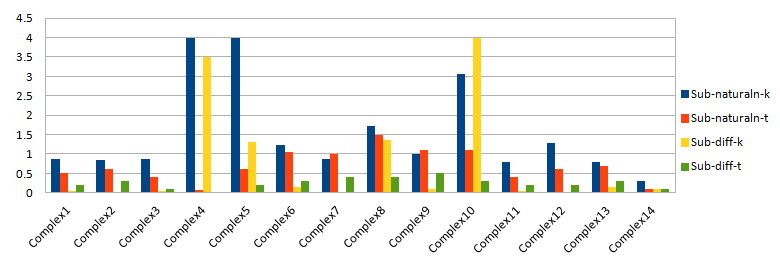
\includegraphics[width=\linewidth]{bar2.png}
\caption{Subjective factors comparison}
\label{fig:sub2}
\end{figure}

Based on this theoretical analysis, we show that our tool brings time complexity improvements in SPRWeb (derived theoretically), without a decline in its performance quantitatively.  


\section{Pair-wised approach}
\label{Pair-wised apporach}

To evaluate our approach mentioned in section 3.2, we did analysis with two types of web pages - simple web pages and complex web pages. 

\subsection{Simple web pages}
\label{Simple web pages}

We generated simple web pages(Fig 4.3), having 3 colors in its layout with no text or images. Eight color schemes were used to generate 8 different web pages with similar structure. To test the subjectivity response preservation of tools being compared, we chose colors which were situated at extremities of Ou's subjective response model[]. As defined in chapter 2, colors are represented in three subjective response dimensions - activity, temperature and weight. And 8 color schemes were designed with colors at the extremities of subjective response dimensions. 

\begin{figure}
\centering
\begin{subfigure}{.5\textwidth}
  \centering
  
\includegraphics[width=.5\linewidth]{screenshotofsimple1.png}
  \caption{Simple 1}
  \label{fig:sub1}
\end{subfigure}%
\begin{subfigure}{.5\textwidth}
  \centering
  
\includegraphics[width=.5\linewidth]{screenshotofsimple2.png}
  \caption{Simple 2}
  \label{fig:sub2}
\end{subfigure}
\caption{Simple web pages}
\label{fig:test}
\end{figure}


Our tool and SPRWeb were compared this time on same metrics that were followed in section 4.1 and using the same method. Table 4.2 shows the testing results for simple web pages. 


\begin{table}[!htb]
\caption{Evaluation: Our approach (numbers in scaled CIELAB euclidean distance)}
% title of Table
\centering
% used for centering table
\begin{tabular}{c c c c c c c c c c c}
% centered columns (4 columns)
\hline\hline
%inserts double horizontal lines
Web Page & C\# & P\# & N-S & N-t & D-S & D-t & SN-S & SN-t & SD-S & SD-t\\ [0.5ex]
% inserts table
%heading
\hline
Simple 1&3&2&44.89&52.02&5.78&0.11&0.06&0.29&2.84&3.07\\
Simple 2&3&2&19.23&20.37&4.35&0.04&1.02&0.63&1.74&1.82\\
Simple 3&3&2&78.11&71.24&7.66&0.09&1.08&0.76&2.03&2.54\\
Simple 4&3&2&21.03&30.27&14.19&0.006&1.87&1.92&0.95&1.25\\
Simple 5&3&2&74.7&59.76&0.33&0.15&1.1&2.05&3.38&3.26\\
Simple 6&3&2&20.41&28.16&0.11&0.009&1.43&1.66&1.8&1.94\\
Simple 7&3&2&63.46&78.98&0.003&0.13&2.31&2.52&2.57&2.73\\
Simple 8&3&2&24.67&38.17&8.35&0.04&2.44&2.95&1.29&1.37\\[1ex]
\hline
%inserts single line
\end{tabular}
\label{table:nonlin}
\begin{tabular}{@{}>{$}l<{$}l@{}}
    $S$ & SPRWeb\\
    $t$ & Our tool developed on parsing pairs of colors concept\\
    $N$ & Naturalness\\
    $D$ & Differentiability\\
    $SN$ & Subjective Naturalness\\
    $SD$ & Subjective Differentiability\\
  \end{tabular}
% is used to refer this table in the text
\end{table}

A comparison graph is given in Fig 4.4 (perceptual) and Fig 4.5(subjective).

\begin{figure}[!htb]
  \centering
  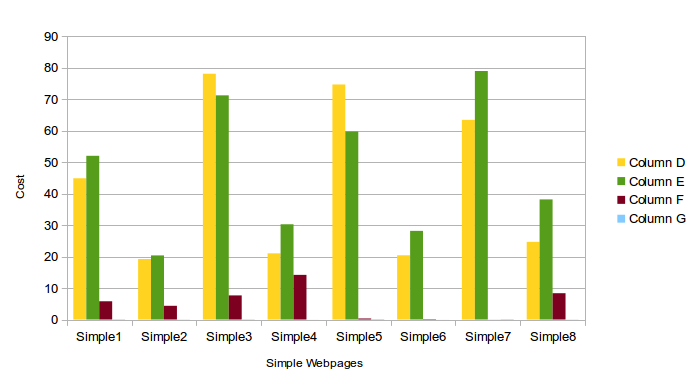
\includegraphics[width=\linewidth]{SimpleGP.png}
  \caption{Perceptual comparison}
  \label{fig:sub1}
\end{figure}

\begin{figure}[!htb]
  \centering
  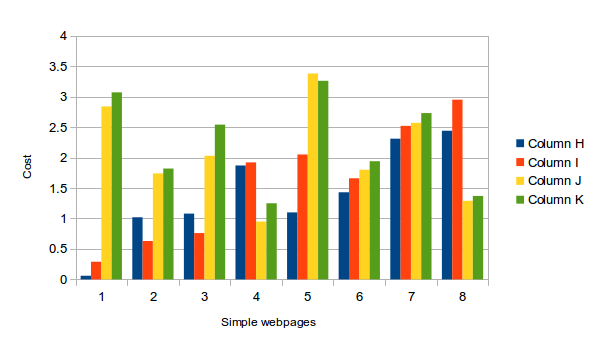
\includegraphics[width=\linewidth]{simpleGS.png}
  \caption{Subjective comparison}
  \label{fig:sub2}
\end{figure}


We also randomly generated 10 simple web pages to compare our tool with SPRWeb. The data is given in Table 4.3.

\begin{table}[!htb]
\caption{Evaluation: Our approach (numbers in scaled CIELAB euclidean distance)}
% title of Table
\centering
% used for centering table
\begin{tabular}{c c c c c c c c c c c}
% centered columns (4 columns)
\hline\hline
%inserts double horizontal lines
Web Page & C\# & P\# & N-S & N-t & D-S & D-t & SN-S & SN-t & SD-S & SD-t\\ [0.5ex]
% inserts table
%heading
\hline
Simple 1&3&2&16.6&15.51&0.04&0.04&1.77&1.27&0.83&0.74\\
Simple 2&3&2&25.2&21.91&0.15&0.02&0.42&0.36&0.05&0.62\\
Simple 3&3&2&24.96&23.76&0.2&0.18&0.24&0.39&0.75&0.65\\
Simple 4&3&2&15.78&72.16&0.06&0.08&0.08&2.05&0.75&1.6\\
Simple 5&3&2&29.33&29.58&10.43&0.14&0.08&0.36&0.92&0.95\\
Simple 6&3&2&46.21&38.87&0.23&0.11&1.26&2.1&1.48&1.73\\
Simple 7&3&2&44.58&40.93&0.18&0.02&0.05&1.12&1.47&1.71\\
Simple 8&3&2&26.89&27.62&5.11&0.04&0.52&0.57&0.9&0.95\\
Simple 9&3&2&25.87&28.14&0.08&0.14&1.41&0.5&0.77&0.96\\
Simple 10&3&2&16.14&17.81&6.76&0.02&0.4&0.33&0.54&0.63\\[1ex]
\hline
%inserts single line
\end{tabular}
\label{table:nonlin}
\begin{tabular}{@{}>{$}l<{$}l@{}}
    $S$ & SPRWeb\\
    $t$ & Our tool developed on parsing pairs of colors concept\\
    $N$ & Naturalness\\
    $D$ & Differentiability\\
    $SN$ & Subjective Naturalness\\
    $SD$ & Subjective Differentiability\\
  \end{tabular}
% is used to refer this table in the text
\end{table}

A comparison plot is given in Fig 4.6 (perceptual) and Fig 4.7 (Subjective). 


\begin{figure}[!htb]
\centering
  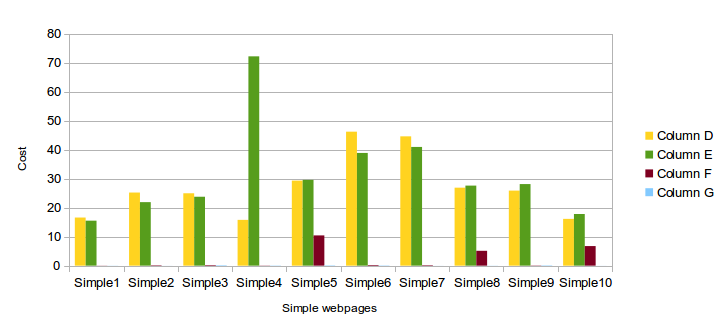
\includegraphics[width=\linewidth]{simpleRP.png}
  \caption{Perceptual comparison}
  \label{fig:sub1}
\end{figure}

\begin{figure}[!htb]
  \centering
  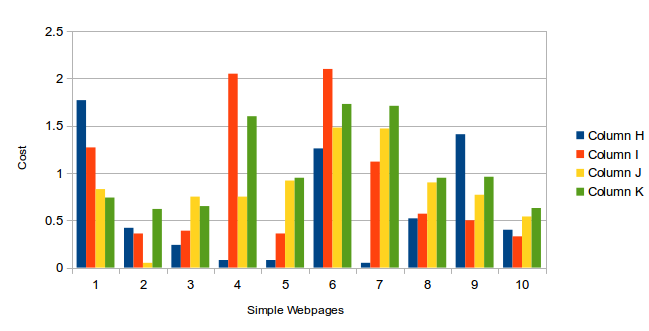
\includegraphics[width=\linewidth]{simpleRS.png}
\caption{Subjective comparison}
\label{fig:test}
\end{figure}

Comparison of total cost can be seen in Fig 4.8 and Fig 4.9 for general and randomly generated web pages respectively. 


\begin{figure}[!htb]
\centering
  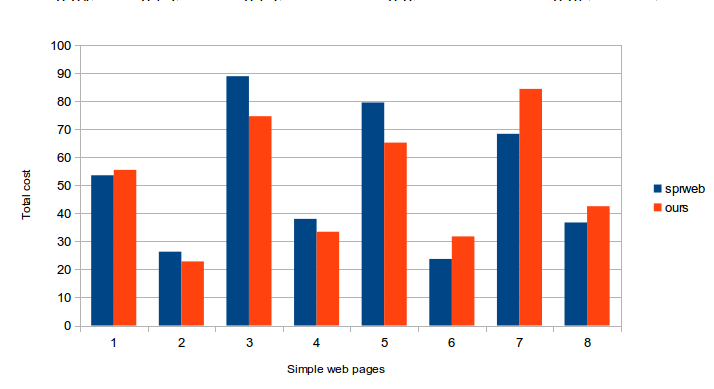
\includegraphics[width=\linewidth]{simpleGtotal.png}
  \caption{Total cost comparison for general pages}
  \label{fig:sub1}
\end{figure}

\begin{figure}[!htb]
  \centering
  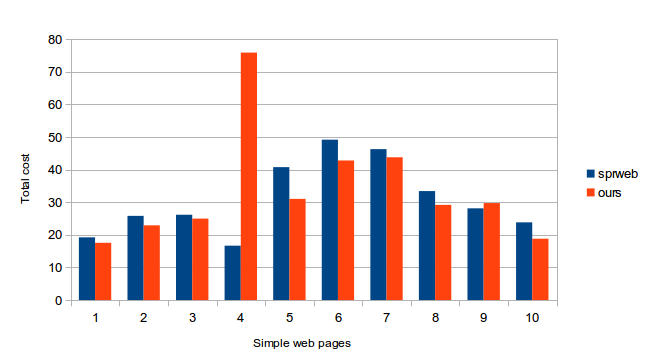
\includegraphics[width=\linewidth]{simpleRtotal.png}
\caption{Total cost comparison for random pages}
\label{fig:test}
\end{figure}


It can be observed from the comparison that our tool performs better in maintaining perceptual differentiability in every case. The overall cost of our tool is less than that of SPRWeb in 12 out of 18 simple web pages. In 2 pages the cost is marginally greater than SPRWeb. It can also be observed that perceptual naturalness cost is significantly higher in our tool as compared to SPRWeb. This can be attributed to the step in the algorithm where we restrict our possible replacement set in order to preserve perceptual differentiability. 


\subsection{Complex web pages}
\label{Complex web pages}
In order to test our tool on real web pages, we selected 14 complex web pages. These web pages consisted of information style pages, forum-style pages and blog style pages. The evaluation data corresponding to these web pages is shown in Table 4.4. 
To test our tool further, we selected 18 more random complex pages and did analysis. Data corresponding to these 18 web pages is shown in Table 4.5. 


\begin{table}[!htb]
\caption{Evaluation: Our approach (numbers in scaled CIELAB euclidean distance)}
% title of Table
\centering
% used for centering table
\begin{tabular}{c c c c c c c c c c c}
% centered columns (4 columns)
\hline\hline
%inserts double horizontal lines
Web Page & C\# & P\# & N-S & N-t & D-S & D-t & SN-S & SN-t & SD-S & SD-t\\ [0.5ex]
% inserts table
%heading
\hline
Complex 1&12&12&29.05&29.05&8.22&0.05&1.08&2.11&1.21&1.26\\
Complex 2&12&9&10.28&11.18&5.08&0.11&1.29&0.94&0.73&0.72\\
Complex 3&4&3&9.15&7.77&0.24&0.1&0.41&0.65&0.28&0.32\\
Complex 4&6&4&7.88&8.66&5.12&0.02&0.31&0.11&0.3&0.39\\
Complex 5&6&4&10.78&10.49&0.079&0.015&0.35&0.71&0.28&0.34\\
Complex 6&7&4&10.19&9.73&2.63&0.05&1.38&2.16&0.92&0.92\\
Complex 7&22&22&21.57&23.99&67.46&0.01&7.35&8.89&1.39&1.48\\
Complex 8&5&4&34.81&46.3&22.7&0.02&1.1&2.32&1.85&2.5\\
Complex 9&7&5&32.5&34.83&28.22&0.08&2.25&0.705&1.57&1.61\\
Complex 10&6&5&13.09&17.29&17.25&0.05&1.68&0.54&0.71&0.649\\
Complex 11&15&15&25.12&27.79&9.88&0.61&0.87&1.15&3.28&4.52\\
Complex 12&13&9&24.45&30.98&15.38&0.24&0.8&1.1&0.9&0.4\\
Complex 13&9&7&13.56&21.33&1.62&0.002&0.77&1.1&1.21&0.62\\
Complex 14&13&10&16.76&17.6&41.62&0.09&0.78&0.82&0.82&0.06\\[1ex]
\hline
%inserts single line
\end{tabular}
\label{table:nonlin}
\begin{tabular}{@{}>{$}l<{$}l@{}}
    $S$ & SPRWeb\\
    $t$ & Our tool developed on parsing pairs of colors concept\\
    $N$ & Naturalness\\
    $D$ & Differentiability\\
    $SN$ & Subjective Naturalness\\
    $SD$ & Subjective Differentiability\\
  \end{tabular}
% is used to refer this table in the text
\end{table}


\begin{table}[!htb]
\caption{Evaluation: Our approach (numbers in scaled CIELAB euclidean distance)}
% title of Table
\centering
% used for centering table
\begin{tabular}{c c c c c c c c c c c}
% centered columns (4 columns)
\hline\hline
%inserts double horizontal lines
Web Page & C\# & P\# & N-S & N-t & D-S & D-t & SN-S & SN-t & SD-S & SD-t\\ [0.5ex]
% inserts table
%heading
\hline
Complex 1&5&3&9.92&9.65&2.49&0.14&1.09&1.02&0.72&0.77\\
Complex 2&10&9&17.51&18.68&40.7&0.08&2.9&1.62&0.87&1.06\\
Complex 3&12&11&29.15&33.21&133.05&0.44&6.33&2.02&1.41&1.46\\
Complex 4&16&17&15.79&15.95&36.8&0.06&4.6&4.02&0.89&0.9\\
Complex 5&8&7&30.22&46.14&69.48&0.35&7.41&6.34&1.62&1.91\\
Complex 6&11&9&1.92&2.19&0.48&0.14&5&5.54&0.48&0.5\\
Complex 7&15&8&11.57&12.44&1.89&0.03&0.91&0.69&1.17&1.18\\
Complex 8&11&12&3.2&3.26&0.56&0.05&0.73&0.11&0.2&0.36\\
Complex 9&8&10&10.39&21.05&20.98&0.24&0.39&6.25&0.83&1.03\\
Complex 10&15&11&24.99&33.76&61.53&0.01&4.6&4.94&1.41&1.78\\
Complex 11&8&9&8.76&9.38&2.34&0.15&0.49&0.68&0.61&0.65\\
Complex 12&16&17&12.73&12.69&14.98&0.4&6.35&5.35&0.87&0.94\\
Complex 13&13&15&3.57&3.7&0.71&0.005&1.01&6.65&0.1&0.24\\
Complex 14&16&12&0.14&0.41&0.089&0.45&0.029&0.86&0.003&0.11\\
Complex 15&10&9&20.62&24.46&1.21&0.03&1.6&1.81&0.99&1.31\\
Complex 16&16&10&22.21&32.2&26.85&0.1&1.23&2.84&1.09&1.42\\
Complex 17&3&3&1.61&12.57&0.32&0.042&0.06&2.51&0.09&0.49\\
Complex 18&16&11&5.33&5.99&0.24&0.4&1.35&2.16&0.16&0.33\\[1ex]
\hline
%inserts single line
\end{tabular}
\label{table:nonlin}
\begin{tabular}{@{}>{$}l<{$}l@{}}
    $S$ & SPRWeb\\
    $t$ & Our tool developed on parsing pairs of colors concept\\
    $N$ & Naturalness\\
    $D$ & Differentiability\\
    $SN$ & Subjective Naturalness\\
    $SD$ & Subjective Differentiability\\
  \end{tabular}
% is used to refer this table in the text
\end{table}

The comparison graphs are provided in Fig 4.10 (general perceptual), Fig 4.11 (general subjective), Fig 4.12 (random perceptual) and Fig 4.13 (random subjective).


\begin{figure}[!htb]
\centering
  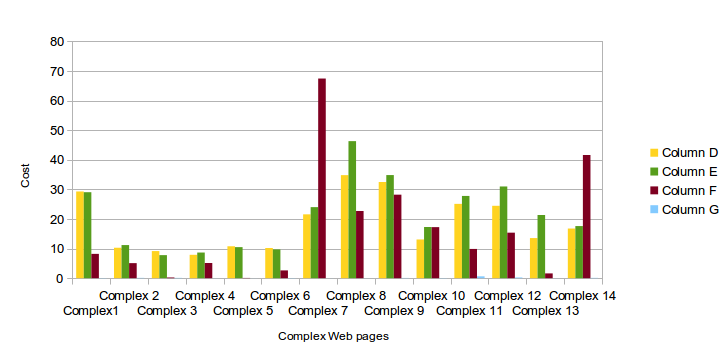
\includegraphics[width=\linewidth]{complexGP.png}
  \caption{Perceptual comparison for general complex pages}
  \label{fig:sub1}
\end{figure}

\begin{figure}[!htb]
  \centering
  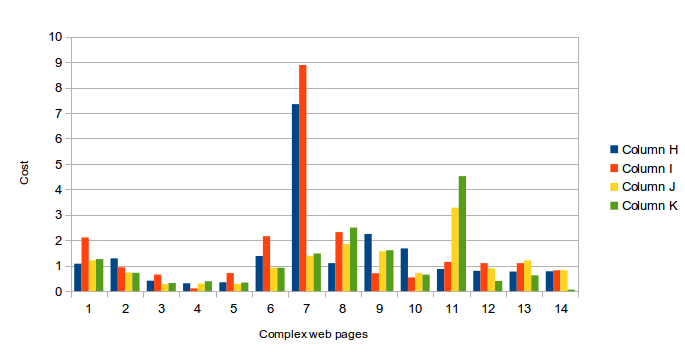
\includegraphics[width=\linewidth]{complexGS.png}
\caption{Subjective comparison for general complex pages}
\label{fig:test}
\end{figure}


\begin{figure}[!htb]
\centering
  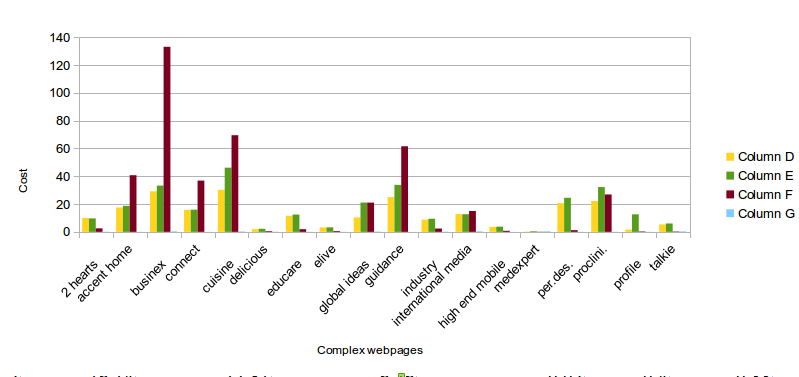
\includegraphics[width=\linewidth]{complexRP.png}
  \caption{Perceptual comparison for random complex pages}
  \label{fig:sub1}
\end{figure}

\begin{figure}[!htb]
  \centering
  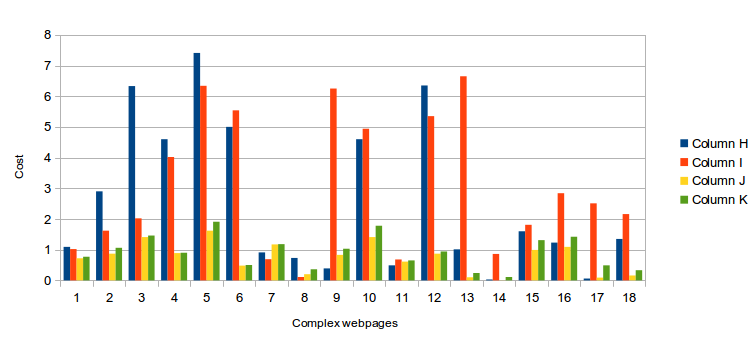
\includegraphics[width=\linewidth]{complexRS.png}
\caption{Subjective comparison for random complex pages}
\label{fig:test}
\end{figure}

Comparison of total cost for both general and random complex pages is provided in Fig 4.14 and Fig 4.15 respectively.

\begin{figure}[!htb]
\centering
  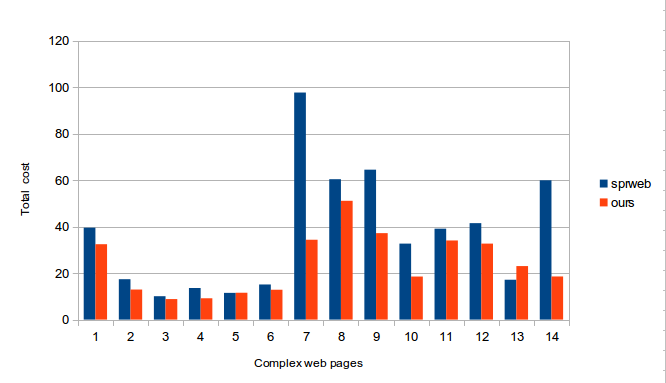
\includegraphics[width=\linewidth]{complexGtotal.png}
  \caption{Total cost comparison for general complex pages}
  \label{fig:sub1}
\end{figure}

\begin{figure}[!htb]
  \centering
  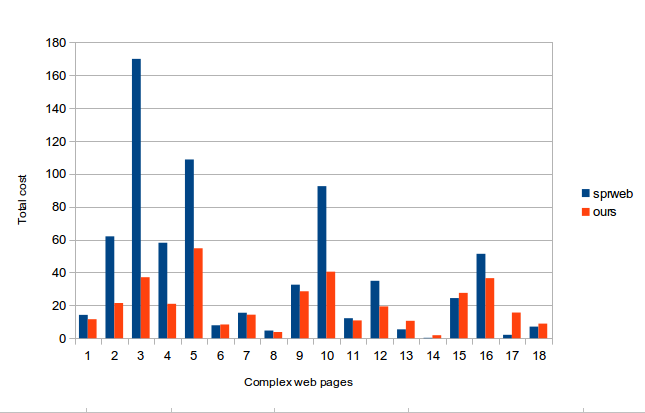
\includegraphics[width=\linewidth]{complexRtotal.png}
\caption{Total cost comparison for random complex pages}
\label{fig:test}
\end{figure}  

By analyzing the total cost comparison for complex web pages, we found that out of 32 pages, our tool performs better in 25 pages. While performs slightly poorer than SPRWeb in 4 pages. It can be observed that while the perceptual differentiability is better in every case for our tool and naturalness suffers. 

\section{Minimum Contrast}
\label{Minimum Contrast}



\subsection{SECTION-TITLE}
\label{SECTION-LABEL}

\subsection{SECTION-TITLE}
\label{SECTION-LABEL}
